\documentclass[portrait,a0paper]{baposter-templ/baposter}

\tracingstats=2

\usepackage{graphicx}
\usepackage{amsmath}
\usepackage{amssymb}
\usepackage{relsize}
\usepackage{multirow}
\usepackage{bm}
\usepackage{booktabs}
\usepackage{colortbl}

\usepackage{graphicx}
\usepackage{multicol}

\usepgflibrary{shapes.symbols}
\usetikzlibrary{shapes.geometric}
\usetikzlibrary{positioning}

\usepackage{times}
\usepackage{helvet}
%\usepackage{bookman}
\usepackage{palatino}

\newcommand{\captionfont}{\footnotesize}

\selectcolormodel{cmyk}


\let\polishl\l

%%%%%%%%%%%%%%%%%%%%%%%%%%%%%%%%%%%%%%%%%%%%%%%%%%%%%%%%%%%%%%%%%%%%%%%%%%%%%%%%
%%%% Math symbols used in the text. Shared with paper
%%%%%%%%%%%%%%%%%%%%%%%%%%%%%%%%%%%%%%%%%%%%%%%%%%%%%%%%%%%%%%%%%%%%%%%%%%%%%%%%
\DeclareMathOperator{\x}{\mathbf{x}}
\DeclareMathOperator{\e}{\mathbf{e}}
\DeclareMathOperator{\M}{\mathbf{M}}
\DeclareMathOperator{\w}{\mathbf{w}}
\newcommand{\fix}{\marginpar{FIX}}
\newcommand{\new}{\marginpar{NEW}}
\edef\polishl{\l} 



\RequirePackage{latexsym}
\RequirePackage{amsmath}
\RequirePackage{amssymb} 
\RequirePackage{color} 
\RequirePackage{bm}
\RequirePackage{color}
\RequirePackage{picinpar}

%%%%%%%% Stock standard definitions %%%%%%%%%%%%%%%

\newcommand{\wbt}{\widetilde{\mathbf{w}}}
\DeclareMathOperator{\ab}{\mathbf{a}}
\DeclareMathOperator{\abh}{\widehat{\ab}}
\DeclareMathOperator{\bb}{\mathbf{b}}
\DeclareMathOperator{\bbh}{\widehat{\bb}}
\DeclareMathOperator{\cb}{\mathbf{c}}
\DeclareMathOperator{\db}{\mathbf{d}}
\DeclareMathOperator{\eb}{\mathbf{e}}
\DeclareMathOperator{\fb}{\mathbf{f}}
\DeclareMathOperator{\gb}{\mathbf{g}}
\DeclareMathOperator{\hb}{\mathbf{h}}
\DeclareMathOperator{\ib}{\mathbf{i}}
\DeclareMathOperator{\jb}{\mathbf{j}}
\DeclareMathOperator{\kb}{\mathbf{k}}
\DeclareMathOperator{\lb}{\mathbf{l}}
\DeclareMathOperator{\mb}{\mathbf{m}}
\DeclareMathOperator{\nbb}{\mathbf{n}}
\DeclareMathOperator{\ob}{\mathbf{o}}
\DeclareMathOperator{\pb}{\mathbf{p}}
\DeclareMathOperator{\qb}{\mathbf{q}}
\DeclareMathOperator{\rb}{\mathbf{r}}
\DeclareMathOperator{\sbb}{\mathbf{s}}
\DeclareMathOperator{\tb}{\mathbf{t}}
\DeclareMathOperator{\ub}{\mathbf{u}}
\DeclareMathOperator{\vb}{\mathbf{v}}
\DeclareMathOperator{\wb}{\mathbf{w}}
\DeclareMathOperator{\xb}{\mathbf{x}}
\DeclareMathOperator{\yb}{\mathbf{y}}
\DeclareMathOperator{\zb}{\mathbf{z}}
\renewcommand{\l}{\ell}

\DeclareMathOperator{\atilde}{\tilde{\ab}}
\DeclareMathOperator{\btilde}{\tilde{\bb}}
\DeclareMathOperator{\ctilde}{\tilde{\cb}}
\DeclareMathOperator{\dtilde}{\tilde{\db}}
\DeclareMathOperator{\etilde}{\tilde{\eb}}
\DeclareMathOperator{\ftilde}{\tilde{\fb}}
\DeclareMathOperator{\gtilde}{\tilde{\gb}}
\DeclareMathOperator{\htilde}{\tilde{\hb}}
\DeclareMathOperator{\itilde}{\tilde{\ib}}
\DeclareMathOperator{\jtilde}{\tilde{\jb}}
\DeclareMathOperator{\ktilde}{\tilde{\kb}}
\DeclareMathOperator{\ltilde}{\tilde{\lb}}
\DeclareMathOperator{\mtilde}{\tilde{\mb}}
\DeclareMathOperator{\ntilde}{\tilde{\nbb}}
\DeclareMathOperator{\otilde}{\tilde{\ob}}
\DeclareMathOperator{\ptilde}{\tilde{\pb}}
\DeclareMathOperator{\qtilde}{\tilde{\qb}}
\DeclareMathOperator{\rtilde}{\tilde{\rb}}
\DeclareMathOperator{\stilde}{\tilde{\sbb}}
\DeclareMathOperator{\ttilde}{\tilde{\tb}}
\DeclareMathOperator{\utilde}{\tilde{\ub}}
\DeclareMathOperator{\vtilde}{\tilde{\vb}}
\DeclareMathOperator{\wtilde}{\tilde{\wb}}
\DeclareMathOperator{\xtilde}{\tilde{\xb}}
\DeclareMathOperator{\ytilde}{\tilde{\yb}}
\DeclareMathOperator{\ztilde}{\tilde{\zb}}

\DeclareMathOperator{\abar}{\bar{\ab}}
\DeclareMathOperator{\bbar}{\bar{\bb}}
\DeclareMathOperator{\cbar}{\bar{\cb}}
\DeclareMathOperator{\dbar}{\bar{\db}}
\DeclareMathOperator{\ebar}{\bar{\eb}}
\DeclareMathOperator{\fbar}{\bar{\fb}}
\DeclareMathOperator{\gbar}{\bar{\gb}}
\DeclareMathOperator{\hbbar}{\bar{\hb}}
\DeclareMathOperator{\ibar}{\bar{\ib}}
\DeclareMathOperator{\jbar}{\bar{\jb}}
\DeclareMathOperator{\kbar}{\bar{\kb}}
\DeclareMathOperator{\lbar}{\bar{\lb}}
\DeclareMathOperator{\mbar}{\bar{\mb}}
\DeclareMathOperator{\nbar}{\bar{\nbb}}
\DeclareMathOperator{\obar}{\bar{\ob}}
\DeclareMathOperator{\pbar}{\bar{\pb}}
\DeclareMathOperator{\qbar}{\bar{\qb}}
\DeclareMathOperator{\rbar}{\bar{\rb}}
\DeclareMathOperator{\sbar}{\bar{\sbb}}
\DeclareMathOperator{\tbar}{\bar{\tb}}
\DeclareMathOperator{\ubar}{\bar{\ub}}
\DeclareMathOperator{\vbar}{\bar{\vb}}
\DeclareMathOperator{\wbar}{\bar{\wb}}
\DeclareMathOperator{\xbar}{\bar{\xb}}
\DeclareMathOperator{\ybar}{\bar{\yb}}
\DeclareMathOperator{\zbar}{\bar{\zb}}

\DeclareMathOperator{\Ab}{\mathbf{A}}
\DeclareMathOperator{\Bb}{\mathbf{B}}
\DeclareMathOperator{\Cb}{\mathbf{C}}
\DeclareMathOperator{\Db}{\mathbf{D}}
\DeclareMathOperator{\Eb}{\mathbf{E}}
\DeclareMathOperator{\Fb}{\mathbf{F}}
\DeclareMathOperator{\Gb}{\mathbf{G}}
\DeclareMathOperator{\Hb}{\mathbf{H}}
\DeclareMathOperator{\Ib}{\mathbf{I}}
\DeclareMathOperator{\Jb}{\mathbf{J}}
\DeclareMathOperator{\Kb}{\mathbf{K}}
\DeclareMathOperator{\Lb}{\mathbf{L}}
\DeclareMathOperator{\Mb}{\mathbf{M}}
\DeclareMathOperator{\Nb}{\mathbf{N}}
\DeclareMathOperator{\Ob}{\mathbf{O}}
\DeclareMathOperator{\Pb}{\mathbf{P}}
\DeclareMathOperator{\Qb}{\mathbf{Q}}
\DeclareMathOperator{\Rb}{\mathbf{R}}
\DeclareMathOperator{\Sbb}{\mathbf{S}}
\DeclareMathOperator{\Tb}{\mathbf{T}}
\DeclareMathOperator{\Ub}{\mathbf{U}}
\DeclareMathOperator{\Vb}{\mathbf{V}}
\DeclareMathOperator{\Wb}{\mathbf{W}}
\DeclareMathOperator{\Xb}{\mathbf{X}}
\DeclareMathOperator{\Xbt}{\widetilde{\Xb}}
\DeclareMathOperator{\Xbh}{\widehat{\Xb}}
\DeclareMathOperator{\Xbs}{\widetilde{\Xb}}
\DeclareMathOperator{\Zbs}{\widetilde{\Zb}}
\DeclareMathOperator{\Kbs}{\widetilde{\Kb}}
\DeclareMathOperator{\Zbh}{\widehat{\Zb}}
\DeclareMathOperator{\Ubh}{\widehat{\Ub}}
\DeclareMathOperator{\Yb}{\mathbf{Y}}
\DeclareMathOperator{\Zb}{\mathbf{Z}}

\DeclareMathOperator{\Abar}{\bar{A}}
\DeclareMathOperator{\Bbar}{\bar{B}}
\DeclareMathOperator{\Cbar}{\bar{C}}
\DeclareMathOperator{\Dbar}{\bar{D}}
\DeclareMathOperator{\Ebar}{\bar{E}}
\DeclareMathOperator{\Fbar}{\bar{F}}
\DeclareMathOperator{\Gbar}{\bar{G}}
\DeclareMathOperator{\Hbar}{\bar{H}}
\DeclareMathOperator{\Ibar}{\bar{I}}
\DeclareMathOperator{\Jbar}{\bar{J}}
\DeclareMathOperator{\Kbar}{\bar{K}}
\DeclareMathOperator{\Lbar}{\bar{L}}
\DeclareMathOperator{\Mbar}{\bar{M}}
\DeclareMathOperator{\Nbar}{\bar{N}}
\DeclareMathOperator{\Obar}{\bar{O}}
\DeclareMathOperator{\Pbar}{\bar{P}}
\DeclareMathOperator{\Qbar}{\bar{Q}}
\DeclareMathOperator{\Rbar}{\bar{R}}
\DeclareMathOperator{\Sbar}{\bar{S}}
\DeclareMathOperator{\Tbar}{\bar{T}}
\DeclareMathOperator{\Ubar}{\bar{U}}
\DeclareMathOperator{\Vbar}{\bar{V}}
\DeclareMathOperator{\Wbar}{\bar{W}}
\DeclareMathOperator{\Xbar}{\bar{X}}
\DeclareMathOperator{\Ybar}{\bar{Y}}
\DeclareMathOperator{\Zbar}{\bar{Z}}

\DeclareMathOperator{\Abbar}{\bar{\Ab}}
\DeclareMathOperator{\Bbbar}{\bar{\Bb}}
\DeclareMathOperator{\Cbbar}{\bar{\Cb}}
\DeclareMathOperator{\Dbbar}{\bar{\Db}}
\DeclareMathOperator{\Ebbar}{\bar{\Eb}}
\DeclareMathOperator{\Fbbar}{\bar{\Fb}}
\DeclareMathOperator{\Gbbar}{\bar{\Gb}}
\DeclareMathOperator{\Hbbar}{\bar{\Hb}}
\DeclareMathOperator{\Ibbar}{\bar{\Ib}}
\DeclareMathOperator{\Jbbar}{\bar{\Jb}}
\DeclareMathOperator{\Kbbar}{\bar{\Kb}}
\DeclareMathOperator{\Lbbar}{\bar{\Lb}}
\DeclareMathOperator{\Mbbar}{\bar{\Mb}}
\DeclareMathOperator{\Nbbar}{\bar{\Nb}}
\DeclareMathOperator{\Obbar}{\bar{\Ob}}
\DeclareMathOperator{\Pbbar}{\bar{\Pb}}
\DeclareMathOperator{\Qbbar}{\bar{\Qb}}
\DeclareMathOperator{\Rbbar}{\bar{\Rb}}
\DeclareMathOperator{\Sbbar}{\bar{\Sb}}
\DeclareMathOperator{\Tbbar}{\bar{\Tb}}
\DeclareMathOperator{\Ubbar}{\bar{\Ub}}
\DeclareMathOperator{\Vbbar}{\bar{\Vb}}
\DeclareMathOperator{\Wbbar}{\bar{\Wb}}
\DeclareMathOperator{\Xbbar}{\bar{\Xb}}
\DeclareMathOperator{\Ybbar}{\bar{\Yb}}
\DeclareMathOperator{\Zbbar}{\bar{\Zb}}

\DeclareMathOperator{\Ahat}{\widehat{A}}
\DeclareMathOperator{\Bhat}{\widehat{B}}
\DeclareMathOperator{\Chat}{\widehat{C}}
\DeclareMathOperator{\Dhat}{\widehat{D}}
\DeclareMathOperator{\Ehat}{\widehat{E}}
\DeclareMathOperator{\Fhat}{\widehat{F}}
\DeclareMathOperator{\Ghat}{\widehat{G}}
\DeclareMathOperator{\Hhat}{\widehat{H}}
\DeclareMathOperator{\Ihat}{\widehat{I}}
\DeclareMathOperator{\Jhat}{\widehat{J}}
\DeclareMathOperator{\Khat}{\widehat{K}}
\DeclareMathOperator{\Lhat}{\widehat{L}}
\DeclareMathOperator{\Mhat}{\widehat{M}}
\DeclareMathOperator{\Nhat}{\widehat{N}}
\DeclareMathOperator{\Ohat}{\widehat{O}}
\DeclareMathOperator{\Phat}{\widehat{P}}
\DeclareMathOperator{\Qhat}{\widehat{Q}}
\DeclareMathOperator{\Rhat}{\widehat{R}}
\DeclareMathOperator{\Shat}{\widehat{S}}
\DeclareMathOperator{\That}{\widehat{T}}
\DeclareMathOperator{\Uhat}{\widehat{U}}
\DeclareMathOperator{\Vhat}{\widehat{V}}
\DeclareMathOperator{\What}{\widehat{W}}
\DeclareMathOperator{\Xhat}{\widehat{X}}
\DeclareMathOperator{\Yhat}{\widehat{Y}}
\DeclareMathOperator{\Zhat}{\widehat{Z}}

\DeclareMathOperator{\Abhat}{\widehat{\Ab}}
\DeclareMathOperator{\Bbhat}{\widehat{\Bb}}
\DeclareMathOperator{\Cbhat}{\widehat{\Cb}}
\DeclareMathOperator{\Dbhat}{\widehat{\Db}}
\DeclareMathOperator{\Ebhat}{\widehat{\Eb}}
\DeclareMathOperator{\Fbhat}{\widehat{\Fb}}
\DeclareMathOperator{\Gbhat}{\widehat{\Gb}}
\DeclareMathOperator{\Hbhat}{\widehat{\Hb}}
\DeclareMathOperator{\Ibhat}{\widehat{\Ib}}
\DeclareMathOperator{\Jbhat}{\widehat{\Jb}}
\DeclareMathOperator{\Kbhat}{\widehat{\Kb}}
\DeclareMathOperator{\Lbhat}{\widehat{\Lb}}
\DeclareMathOperator{\Mbhat}{\widehat{\Mb}}
\DeclareMathOperator{\Nbhat}{\widehat{\Nb}}
\DeclareMathOperator{\Obhat}{\widehat{\Ob}}
\DeclareMathOperator{\Pbhat}{\widehat{\Pb}}
\DeclareMathOperator{\Qbhat}{\widehat{\Qb}}
\DeclareMathOperator{\Rbhat}{\widehat{\Rb}}
\DeclareMathOperator{\Sbhat}{\widehat{\Sb}}
\DeclareMathOperator{\Tbhat}{\widehat{\Tb}}
\DeclareMathOperator{\Ubhat}{\widehat{\Ub}}
\DeclareMathOperator{\Vbhat}{\widehat{\Vb}}
\DeclareMathOperator{\Wbhat}{\widehat{\Wb}}
\DeclareMathOperator{\Xbhat}{\widehat{\Xb}}
\DeclareMathOperator{\Ybhat}{\widehat{\Yb}}
\DeclareMathOperator{\Zbhat}{\widehat{\Zb}}

\DeclareMathOperator{\Acal}{\mathcal{A}}
\DeclareMathOperator{\Bcal}{\mathcal{B}}
\DeclareMathOperator{\Ccal}{\mathcal{C}}
\DeclareMathOperator{\Dcal}{\mathcal{D}}
\DeclareMathOperator{\Ecal}{\mathcal{E}}
\DeclareMathOperator{\Fcal}{\mathcal{F}}
\DeclareMathOperator{\Gcal}{\mathcal{G}}
\DeclareMathOperator{\Hcal}{\mathcal{H}}
\DeclareMathOperator{\Ical}{\mathcal{I}}
\DeclareMathOperator{\Jcal}{\mathcal{J}}
\DeclareMathOperator{\Kcal}{\mathcal{K}}
\DeclareMathOperator{\Lcal}{\mathcal{L}}
\DeclareMathOperator{\Mcal}{\mathcal{M}}
\DeclareMathOperator{\Ncal}{\mathcal{N}}
\DeclareMathOperator{\Ocal}{\mathcal{O}}
\DeclareMathOperator{\Pcal}{\mathcal{P}}
\DeclareMathOperator{\Qcal}{\mathcal{Q}}
\DeclareMathOperator{\Rcal}{\mathcal{R}}
\DeclareMathOperator{\Scal}{\mathcal{S}}
\DeclareMathOperator{\Scalt}{\widetilde{\Scal}}
\DeclareMathOperator{\Tcal}{\mathcal{T}}
\DeclareMathOperator{\Ucal}{\mathcal{U}}
\DeclareMathOperator{\Vcal}{\mathcal{V}}
\DeclareMathOperator{\Wcal}{\mathcal{W}}
\DeclareMathOperator{\Xcal}{\mathcal{X}}
\DeclareMathOperator{\Ycal}{\mathcal{Y}}
\DeclareMathOperator{\Zcal}{\mathcal{Z}}

\DeclareMathOperator{\Atilde}{\widetilde{A}}
\DeclareMathOperator{\Btilde}{\widetilde{B}}
\DeclareMathOperator{\Ctilde}{\widetilde{C}}
\DeclareMathOperator{\Dtilde}{\widetilde{D}}
\DeclareMathOperator{\Etilde}{\widetilde{E}}
\DeclareMathOperator{\Ftilde}{\widetilde{F}}
\DeclareMathOperator{\Gtilde}{\widetilde{G}}
\DeclareMathOperator{\Htilde}{\widetilde{H}}
\DeclareMathOperator{\Itilde}{\widetilde{I}}
\DeclareMathOperator{\Jtilde}{\widetilde{J}}
\DeclareMathOperator{\Ktilde}{\widetilde{K}}
\DeclareMathOperator{\Ltilde}{\widetilde{L}}
\DeclareMathOperator{\Mtilde}{\widetilde{M}}
\DeclareMathOperator{\Ntilde}{\widetilde{N}}
\DeclareMathOperator{\Otilde}{\widetilde{O}}
\DeclareMathOperator{\Ptilde}{\widetilde{P}}
\DeclareMathOperator{\Qtilde}{\widetilde{Q}}
\DeclareMathOperator{\Rtilde}{\widetilde{R}}
\DeclareMathOperator{\Stilde}{\widetilde{S}}
\DeclareMathOperator{\Ttilde}{\widetilde{T}}
\DeclareMathOperator{\Utilde}{\widetilde{U}}
\DeclareMathOperator{\Vtilde}{\widetilde{V}}
\DeclareMathOperator{\Wtilde}{\widetilde{W}}
\DeclareMathOperator{\Xtilde}{\widetilde{X}}
\DeclareMathOperator{\Ytilde}{\widetilde{Y}}
\DeclareMathOperator{\Ztilde}{\widetilde{Z}}


%%%%%%%% Widely accepted definitions %%%%%%%%%%%%%%%

\DeclareMathOperator{\CC}{\mathbb{C}} % Complex numbers
\DeclareMathOperator{\EE}{\mathbb{E}} % Expectation
\DeclareMathOperator{\KK}{\mathbb{K}} % Arbitrary field
\DeclareMathOperator{\MM}{\mathbb{M}} % Median
\DeclareMathOperator{\NN}{\mathbb{N}} % Natural numbers
\DeclareMathOperator{\PP}{\mathbb{P}} % Probability
\DeclareMathOperator{\QQ}{\mathbb{Q}} % Rationals
\DeclareMathOperator{\RR}{\mathbb{R}} % Real numbers 
\DeclareMathOperator{\ZZ}{\mathbb{Z}} % Integers

\DeclareMathOperator{\one}{\mathbf{1}}  % Identity
\DeclareMathOperator{\zero}{\mathbf{0}} % Zero
\DeclareMathOperator{\TRUE}{\mathbf{TRUE}}  % True
\DeclareMathOperator{\FALSE}{\mathbf{FALSE}}  % False

\DeclareMathOperator*{\mini}{\mathop{\mathrm{minimize}}}
\DeclareMathOperator*{\maxi}{\mathop{\mathrm{maximize}}}
\DeclareMathOperator*{\argmin}{\mathop{\mathrm{argmin}}}
\DeclareMathOperator*{\argmax}{\mathop{\mathrm{argmax}}}
\DeclareMathOperator*{\argsup}{\mathop{\mathrm{argsup}}}
\DeclareMathOperator*{\arginf}{\mathop{\mathrm{arginf}}}
\DeclareMathOperator{\sgn}{\mathop{\mathrm{sign}}}
\DeclareMathOperator{\sign}{\mathop{\mathrm{sign}}}
\DeclareMathOperator{\tr}{\mathop{\mathrm{tr}}}
\DeclareMathOperator{\rank}{\mathop{\mathrm{rank}}}
\DeclareMathOperator{\traj}{\mathop{\mathrm{Traj}}}

%%%%%%%% Bold Greek Letters %%%%%%%%%%%%%%%
\DeclareMathOperator{\sigmab}{\bm{\sigma}}
\DeclareMathOperator{\Sigmab}{\mathbf{\Sigma}}


%%%%%%%% Mess around with LaTeX %%%%%%%%%%%%%%%

%% Some style files might actually define these variables.
%% So don't mess with them if they are already defined

\ifx\BlackBox\undefined
\newcommand{\BlackBox}{\rule{1.5ex}{1.5ex}}  % end of proof
\fi

\ifx\proof\undefined
\newenvironment{proof}{\par\noindent{\bf Proof\ }}{\hfill\BlackBox\\[2mm]}
% \else
% \renewenvironment{proof}{\par\noindent{\bf Proof\ }}{\hfill\BlackBox\\[2mm]}
\fi

%Trying to put all on Section track
%\makeatletter
%\@addtoreset{equation}{section}
%\def\theequation{\thesection.\arabic{equation}}
%\def\thetheorem{\thesection.\arabic{theorem}}
%\makeatother

%the below clashes with the previous defs of them... 
%in the style files
%\newtheorem{theorem}{Theorem}[section]
%\newtheorem{lemma}[theorem]{Lemma}
%\newtheorem{corollary}[theorem]{Corollary}
%\newtheorem{conjecture}[conjecture]{Conjecture}


%%%%%%%% Utility functions %%%%%%%%%%%%%%%

\newcommand{\eq}[1]{(\ref{#1})} 
\newcommand{\mymatrix}[2]{\left[\begin{array}{#1} #2 \end{array}\right]}
\newcommand{\mychoose}[2]{\left(\begin{array}{c} #1 \\ #2 \end{array}\right)}
\newcommand{\mydet}[1]{\det\left[ #1 \right]}
\newcommand{\sembrack}[1]{[\![#1]\!]}

\newcommand{\ea}{\emph{et al. }}
\newcommand{\eg}{\emph{e.g. }}
\newcommand{\ie}{\emph{i.e., }}

\newcommand{\mnote}[1]{\marginpar{#1}}
\newcommand{\note}[1]{{\bf {#1}}}

%%%%%%%% Specific symbols for this project %%%%%%%%%%%%%%%

\DeclareMathOperator{\half}{\frac{1}{2}}

\newcommand{\Ref}[1]{\hfill\Green{[#1]}}
\DeclareMathOperator{\XX}{\mathcal{X}}
\newcommand{\ar}{\implies}
\newcommand{\yh}{\hat{y}}
\DeclareMathOperator{\lan}{\langle}
\DeclareMathOperator{\ran}{\rangle}

\DeclareMathOperator{\dc}{\mathrm{dc}}

\DeclareMathOperator{\Utb}{\widetilde{\Ub}}
\DeclareMathOperator{\Stb}{\widetilde{\Sbb}}

\ifx\Brown\undefined
\definecolor{brown}{rgb}{0.5,0.1,0.1}
\newcommand{\Brown}[1]{\color{brown}{#1}\color{black}}
\fi

\ifx\Red\undefined
\definecolor{red}{rgb}{1.0,0,0}
\newcommand{\Red}[1]{\color{red}{#1}\color{black}}
\fi

\ifx\Green\undefined
\definecolor{green}{rgb}{0,0.4,0}
\newcommand{\Green}[1]{\color{green}{#1}\color{black}}
\fi

\ifx\Blue\undefined
\definecolor{blue}{rgb}{0,0,1.0}
\newcommand{\Blue}[1]{\color{blue}{#1}\color{black}}
\fi



\newcommand{\beq}{\begin{equation}}
\newcommand{\eeq}{\end{equation}}
\newcommand{\beh}{\begin{conjecture}}
\newcommand{\eeh}{\end{conjecture}}
\newcommand\bel{\begin{lemma}}
\newcommand\eel{\end{lemma}}
\newcommand\bet{\begin{theoreme}}
\newcommand\eet{\end{theoreme}}
\newcommand\bex{\begin{example}}
\newcommand\eex{\end{example}}
\newcommand\bed{\begin{definition}}
\newcommand\eed{\end{definition}}
\newcommand\bep{\begin{proposition}}
\newcommand\eep{\end{proposition}}
\newcommand\ber{\begin{remark}}
\newcommand\eer{\end{remark}}
\newcommand\bec{\begin{corollary}}
\newcommand\eec{\end{corollary}}
%\newcommand\proof{\noindent {\bf Proof.}\ \ }
\newcommand\qed{\hfill$\Box$\medskip}
\newcommand\cP{{\mathcal P}}
\newcommand\cJ{{\mathcal J}}
\newcommand\cD{{\mathcal D}}
\newcommand\cC{{\mathcal C}}
\newcommand\cO{{\mathcal O}}
\newcommand\cS{{\mathcal S}}
\newcommand\cT{{\mathcal T}}
\newcommand\cV{{\mathcal V}}
\newcommand\cW{{\mathcal W}}
\newcommand\cY{{\mathcal Y}}
\newcommand\cF{{\mathcal F}}
\newcommand\cU{{\mathcal U}}
\newcommand\cE{{\mathcal E}}
\newcommand\cG{{\mathcal G}}
\newcommand\cB{{\mathcal B}}
\newcommand\cI{{\rm I}}
\newcommand\cN{{\mathcal N}}
\newcommand\cM{{\mathcal M}}
\newcommand\cA{{\mathcal A}}
\newcommand\cQ{{\mathcal Q}}
\newcommand\cK{{\mathcal K}}
\newcommand\cZ{{\mathcal Z}}
\newcommand\CAP{{\rm cap}}
\newcommand\ENT{{\rm ent}}
\newcommand\gr{{\rm gr}}

\def\qq{{\mathbb Q}}
\def\ff{{\mathbb F}}
\def\rr{{\mathbb R}}
\def\zz{{\mathbb Z}}
\def\cc{{\mathbb C}}
\def\nn{{\mathbb N}}
\def\kk{{\mathbb K}}
\def\ee{{\mathbb E}}
\def\ww{{\mathbb W}}
\def\hh{{\mathbb H}}
\def\ss{{\mathbb S}}
\def\tt{{\mathbb T}}
\def\pp{{\mathbb P}}




%%%%%%%%%%%%%%%%%%%%%%%%%%%%%%%%%%%%%%%%%%%%%%%%%%%%%%%%%%%%%%%%%%%%%%%%%%%%%%%%
% Multicol Settings
%%%%%%%%%%%%%%%%%%%%%%%%%%%%%%%%%%%%%%%%%%%%%%%%%%%%%%%%%%%%%%%%%%%%%%%%%%%%%%%%
\setlength{\columnsep}{0.7em}
\setlength{\columnseprule}{0mm}


%%%%%%%%%%%%%%%%%%%%%%%%%%%%%%%%%%%%%%%%%%%%%%%%%%%%%%%%%%%%%%%%%%%%%%%%%%%%%%%%
% Save space in lists. Use this after the opening of the list
%%%%%%%%%%%%%%%%%%%%%%%%%%%%%%%%%%%%%%%%%%%%%%%%%%%%%%%%%%%%%%%%%%%%%%%%%%%%%%%%
\newcommand{\compresslist}{%
\setlength{\itemsep}{1pt}%
\setlength{\parskip}{0pt}%
\setlength{\parsep}{0pt}%
}


%%%%%%%%%%%%%%%%%%%%%%%%%%%%%%%%%%%%%%%%%%%%%%%%%%%%%%%%%%%%%%%%%%%%%%%%%%%%%%
%%% Begin of Document
%%%%%%%%%%%%%%%%%%%%%%%%%%%%%%%%%%%%%%%%%%%%%%%%%%%%%%%%%%%%%%%%%%%%%%%%%%%%%%

\begin{document}

%%%%%%%%%%%%%%%%%%%%%%%%%%%%%%%%%%%%%%%%%%%%%%%%%%%%%%%%%%%%%%%%%%%%%%%%%%%%%%
%%% Here starts the poster
%%%---------------------------------------------------------------------------
%%% Format it to your taste with the options
%%%%%%%%%%%%%%%%%%%%%%%%%%%%%%%%%%%%%%%%%%%%%%%%%%%%%%%%%%%%%%%%%%%%%%%%%%%%%%
% Define some colors
\definecolor{silver}{cmyk}{0,0,0,0.3}
\definecolor{yellow}{cmyk}{0,0,0.9,0.0}
\definecolor{reddishyellow}{cmyk}{0,0.22,1.0,0.0}
\definecolor{black}{cmyk}{0,0,0.0,1.0}
\definecolor{darkYellow}{cmyk}{0,0,1.0,0.5}
\definecolor{darkSilver}{cmyk}{0,0,0,0.1}

\definecolor{lightyellow}{cmyk}{0,0,0.3,0.0}
\definecolor{lighteryellow}{cmyk}{0,0,0.1,0.0}
\definecolor{lightestyellow}{cmyk}{0,0,0.05,0.0}

%%
\typeout{Poster Starts}
\background{}

\newlength{\leftimgwidth}
\begin{poster}%
  % Poster Options
  {
  % Show grid to help with alignment
  grid=false,
  % Column spacing
  colspacing=1em,
  % Color style
  bgColorOne=lighteryellow,
  bgColorTwo=lightestyellow,
  borderColor=reddishyellow,
  headerColorOne=yellow,
  headerColorTwo=reddishyellow,
  headerFontColor=black,
  boxColorOne=lightyellow,
  boxColorTwo=lighteryellow,
  % Format of textbox
  textborder=roundedleft,
%  textborder=rectangle,
  % Format of text header
  eyecatcher=true,
  headerborder=open,
  headerheight=0.09\textheight,
  headershape=roundedright,
  headershade=plain,
  headerfont=\Large\textsf, %Sans Serif
  boxshade=plain,
  background=shadeTB,
  linewidth=2pt
  }
  % Eye Catcher
  {} % No eye catcher for this poster. (eyecatcher=no above). If an eye catcher is present, the title is centered between eye-catcher and logo.
  % Title
  {\sf 
\begin{tabular}{c@{\qquad}c@{\qquad}c}
& An Information Theoretic Approach & \\
\includegraphics[height=1em,viewport=0 160 375 261,clip]{figures/UCSC} 
& to Quantifying Text Interestingness &
\includegraphics[height=1em,viewport=0 160 375 261,clip]{figures/UCSC} 
\end{tabular}
% \footnotesize{%
%  \begin{tabular}{r}NIPS poster\\ Granada 12.12.2011 \end{tabular}
%}
 \vspace{.3em}}
  % Authors
{\sf %Sans Serif
% Serif
\begin{tabular}{c@{\qquad\qquad}c}%@{\qquad\qquad}c}
Micha{\polishl} Derezi\'{n}ski &
Khashayar Rohanimanesh
\\
\end{tabular}
% \raisebox{5mm}{\includegraphics[height=2em,viewport=0 160 375 261,clip]{figures/UCSC}}
%
%
\vspace{-.5em} % bring logos down a bit so title does not touch top
}
% University logo
{}
\tikzstyle{light shaded}=[top color=baposterBGtwo!30!white,bottom color=baposterBGone!30!white,shading=axis,shading angle=30]


%%%%%%%%%%%%%%%%%%%%%%%%%%%%%%%%%%%%%%%%%%%%%%%%%%%%%%%%%%%%%%%%%%%%%%%%%%%%%%
%%% Now define the boxes that make up the poster
%%%---------------------------------------------------------------------------
%%% Each box has a name and can be placed absolutely or relatively.
%%% The only inconvenience is that you can only specify a relative position 
%%% towards an already declared box. So if you have a box attached to the 
%%% bottom, one to the top and a third one which should be in between, you 
%%% have to specify the top and bottom boxes before you specify the middle 
%%% box.
%%%%%%%%%%%%%%%%%%%%%%%%%%%%%%%%%%%%%%%%%%%%%%%%%%%%%%%%%%%%%%%%%%%%%%%%%%%%%%

\fboxsep=0mm%padding thickness
\fboxrule=2pt%border thickness

%%%%%%%%%%%%%%%%%%%%%%%%%%%%%%%%%%%%%%%%%%%%%%%%%%%%%%%%%%%%%%%%%%%%%%%%%%%%%%
\headerbox{Finding Interesting Products}{name=related,column=0,row=0}{
{\bf Goal:} Increase user engagement when shopping on eBay.

\medskip 
{\bf Solution:} Display ads for products that are {\em unique},
  {\em surprising}, {\em interesting}. 

\medskip
Users are unlikely to buy such products, but will spend more time
browsing them and clicking on the ads. 

\vspace{-2mm}
\begin{center}
{\bf Example: Interesting iPhone cases}
\vspace{1mm}

\fcolorbox{reddishyellow}{white}{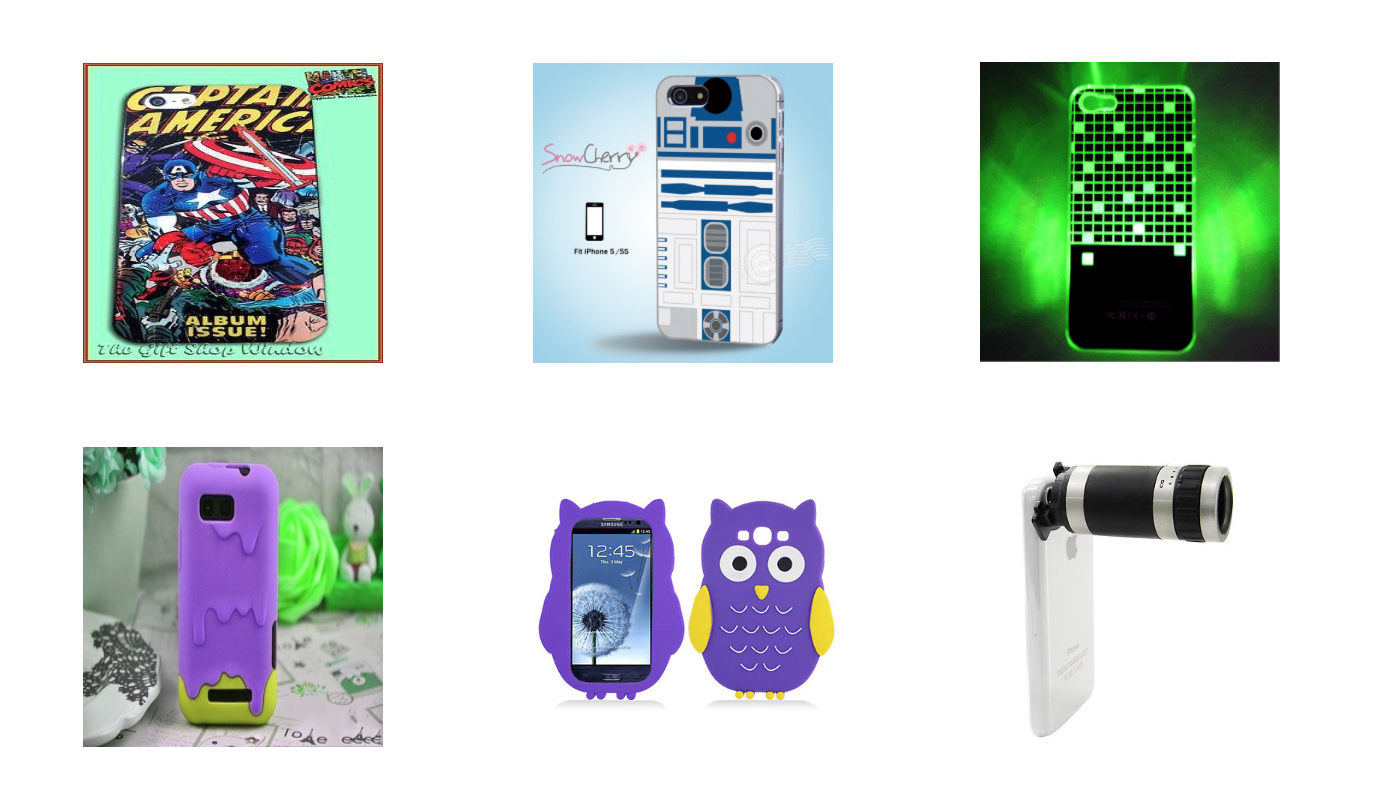
\includegraphics[width=0.95\textwidth]{figures/interesting.png}}
\end{center}
%%%%%%%%%%%%%%%%%%%%%%%%%%%%%%%%%%%%%%%%%%%%%%%%%%%%%%%%%%%%%%%%%%%%%%%%%%%%%% 
 }


%%%%%%%%%%%%%%%%%%%%%%%%%%%%%%%%%%%%%%%%%%%%%%%%%%%%%%%%%%%%%%%%%%%%%%%%%%%%%%
\headerbox{Interestingness as Text Diversity}{name=newcontribution,column=0,below=related}{
We used eBay {\bf product titles as features}.

\medskip
{\bf Hypothesis:} Often an interesting concept is generated
  by mixing a {\bf diverse set of topics}.
We can identify those topics from the words appearing in the
  product title (usually 10-12 words).

\begin{multicols}{2}
\begin{center}\fcolorbox{reddishyellow}{white}{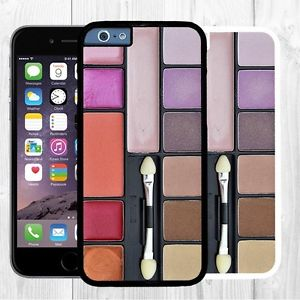
\includegraphics[width=25mm]{figures/eyeshadow-iphone-case.jpg}}
\end{center}

\textcolor{red}{{\bf Eyeshadow}} 
Palettes for \textcolor{red}{{\bf iPhone}} 6 case
\end{multicols}

\begin{multicols}{2}
\begin{center}\fcolorbox{reddishyellow}{white}{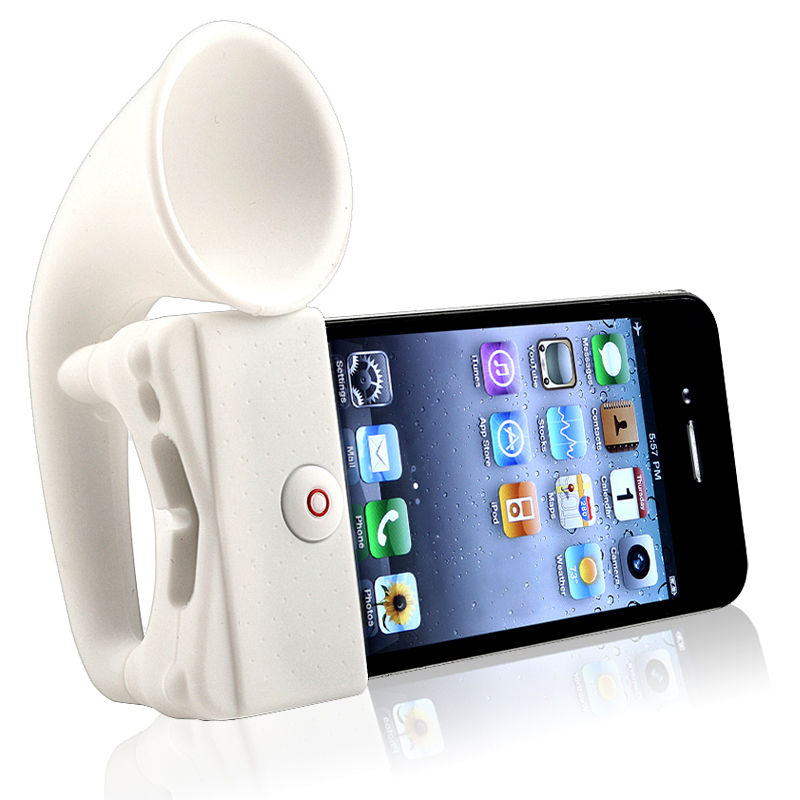
\includegraphics[width=25mm]{figures/horn-iphone-speaker.jpg}} 
\end{center}

White Silicone \textcolor{red}{{\bf Horn}} Stand Speaker for
  Apple \textcolor{red}{{\bf iPhone}} 4/ 4S
\end{multicols}

\begin{multicols}{2}
\begin{center}\fcolorbox{reddishyellow}{white}{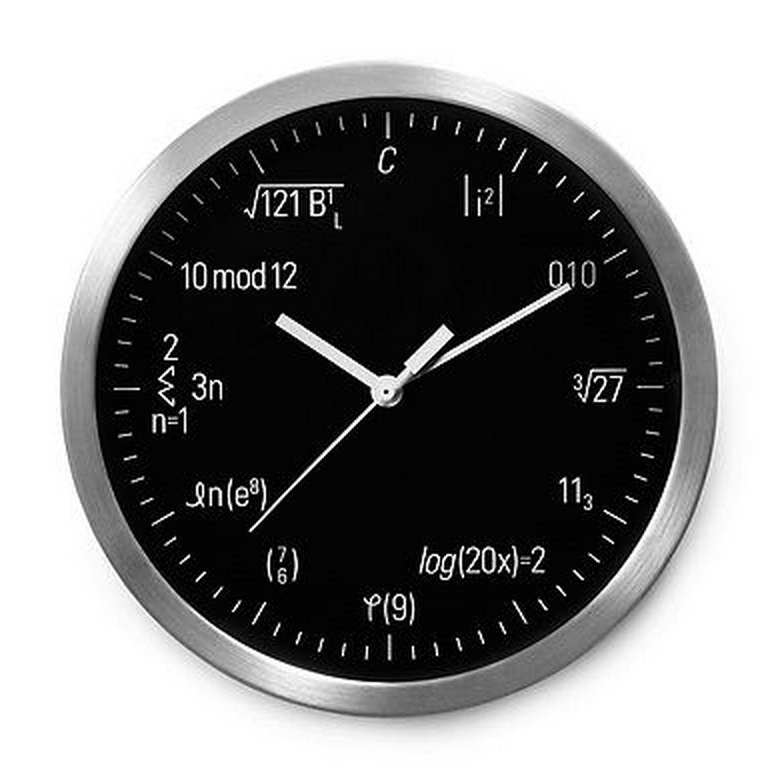
\includegraphics[width=25mm]{figures/geeky-clock.jpg}}
\end{center}

\textcolor{red}{{\bf Equation}} Wall \textcolor{red}{{\bf
      Clock}} Gifts for Math Gurus
\end{multicols}
\vspace{0.0em}
%%%%%%%%%%%%%%%%%%%%%%%%%%%%%%%%%%%%%%%%%%%%%%%%%%%%%%%%%%%%%%%%%%%%%%%%%%%%%% 
 }

%%%%%%%%%%%%%%%%%%%%%%%%%%%%%%%%%%%%%%%%%%%%%%%%%%%%%%%%%%%%%%%%%%%%%%%%%%%%%%
 \headerbox{Data Sets}{name=openproblems,column=0,below=newcontribution,above=bottom}{
{\bf 1. Interesting iPhone cases on eBay.}

We hired workers from {\em AMT} to label a collection
of iPhone cases found on {\em Pinterest} and {\em
  eBay's}. 

The final data-set consists of 2179 positive and 9770
negative instances for 
a total of 11,949 instances, with product title used as input. 
The topic model was trained using Mallet on 2 million product
  titles, grouped by categories into 800 documents.

\medskip
{\bf 2. NSF abstracts (61,902, 200-300 words each).}

We used this set for training a topic model.
To get labeled data, we had to generate $5000$ artificial
  labeled examples, by mixing random abstracts. 
\vspace{0.5em}
%%%%%%%%%%%%%%%%%%%%%%%%%%%%%%%%%%%%%%%%%%%%%%%%%%%%%%%%%%%%%%%%%%%%%%%%%%%%%% 
 }

\newcommand{\AlgShort}{\textsf{Alg}}
\newcommand{\NatShort}{\textsf{Nat}}


%%%%%%%%%%%%%%%%%%%%%%%%%%%%%%%%%%%%%%%%%%%%%%%%%%%%%%%%%%%%%%%%%%%%%%%%%%%%%%
  \headerbox{Words as Topic Distributions}{name=representation,column=1,row=0}{
\setlength{\arrayrulewidth}{2pt} 
\arrayrulecolor{reddishyellow}
\begin{center}
\begin{tabular}{c|ccc}
\rowcolor{yellow} \cellcolor{lightyellow}
$\cM$& {\it Phones} & {\it Computers} & {\it Movies}\\
\hline
\rowcolor{white} \cellcolor{yellow} {\bf iPhone} & 111 & 5 & 1\\
\rowcolor{white} \cellcolor{yellow} {\bf Apple} & 80 & 50 & 0\\
\rowcolor{white} \cellcolor{yellow} {\bf Batman} & 7 & 0 & 65\\
\rowcolor{white} \cellcolor{yellow} {\bf New} & 325 & 240 & 165\\
\rowcolor{white} \cellcolor{yellow} {\bf Esoteric} & 0 & 0 & 1
\end{tabular}
\end{center}

Each word $w_i\in V$ is mapped to a {\bf probability distribution} $P_i$ over topics
$T$, using $\cM$.

% \medskip
% We start from a {\bf co-occurrence matrix} $\cM_{|V|\times|T|}$
%   where each row represents a co-occurrence of a word with the set
%   $T$. For $T=V$, this corresponds to the familiar {\em word-to-word}
%   co-occurrence representation.

 \medskip
 To obtain $\cM$, we use a {\bf topic model} trained with {\em Latent Dirichlet Allocation}. 
 \vspace{0.4em}
%%%%%%%%%%%%%%%%%%%%%%%%%%%%%%%%%%%%%%%%%%%%%%%%%%%%%%%%%%%%%%%%%%%%%%%%%%%%%%
}


%%%%%%%%%%%%%%%%%%%%%%%%%%%%%%%%%%%%%%%%%%%%%%%%%%%%%%%%%%%%%%%%%%%%%%%%%%%%%%
  \headerbox{The Reader's Model}{name=reader,column=2,row=0}{
% Consider a person reading a text $W=\{w_1,...,w_k\}$. 
% The Reader represents the meaning of each word $w_i$ with a probability
%   distribution $P_{i}$ over a set of topics $T$. 
% The Reader's {\em knowledge} is represented by the matrix
% $\cM_{|V|\times|T|}$. Now, we ask:
\begin{center}\fcolorbox{reddishyellow}{white}{
\includegraphics[width=0.95\textwidth]{figures/Books-2-icon-wide.png}}
\end{center}
\vspace{-2mm}
1. Reader chooses $P_{i}$'s for text $W$, knowing $\cM$.

\medskip
2. Having $\cP_{W}=\{P_{1},...,P_{k}\}$, Reader estimates the diversity of $W$.
%%%%%%%%%%%%%%%%%%%%%%%%%%%%%%%%%%%%%%%%%%%%%%%%%%%%%%%%%%%%%%%%%%%%%%%%%%%%%%
}

%%%%%%%%%%%%%%%%%%%%%%%%%%%%%%%%%%%%%%%%%%%%%%%%%%%%%%%%%%%%%%%%%%%%%%%%%%%%%%
\headerbox{Jensen-Shannon Information Diversity}{name=regret,column=1,span=2,below=representation}{
\begin{multicols}{2}
\fboxsep=2pt
\begin{center}\fcolorbox{reddishyellow}{white}{
\parbox{0.45\textwidth}{
{\bf Generalized Jensen-Shannon Divergence} for  $\cP=\{P_{1},...,P_{k}\}$
 and weights $\Sigma d_i=1$ is defined (denoting
 $M=\sum_{i=1}^kd_iP_i$) as  
\vspace{-4mm}
\[D_{JS}(\Sigma d_iP_i) = \sum_{i=1}^k d_i D_{KL}(P_i\|M).\] 
\vspace{-2mm}
}}\end{center}

Here, $D_{KL}$ is the Kullback-Leibler divergence. 

We propose using weights
proportional to the information contained in each distribution. 

\begin{center}\fcolorbox{reddishyellow}{white}{
\parbox{0.45\textwidth}{
Let {\bf importance} of $P_i$ with respect to
prior distribution $P$ be $D_i = D_{KL}(P_i\|P)$. 
}}

\smallskip
\fcolorbox{reddishyellow}{white}{
\parbox{0.45\textwidth}{
We define the {\bf Jensen-Shannon Information Diversity} of $\cP$ with
respect to prior $P$ as $\mbox{JSD}_P(\cP)=D_{JS}(\Sigma d_i P_i)$
where $d_{i}=\frac{D_{i}}{\sum D_{j}}$ are the normalized importances.
}}\end{center}
\end{multicols}
\vspace{0em}
}


%%%%%%%%%%%%%%%%%%%%%%%%%%%%%%%%%%%%%%%%%%%%%%%%%%%%%%%%%%%%%%%%%%%%%%%%%%%%%%
  \headerbox{Choosing Word Representations}{name=dms,column=1,below=regret}{
Given $W=\{w_1,...,w_k\}$, how should the Reader choose $P_{i}$, knowing
  $\cM_{|V|\times|T|}$?

\medskip
{\bf Intuition:} We can use the row of $\cM_{|V|\times|T|}$ that
corresponds to $w_i$, normalized to a distribution.

\medskip
We improve on this approach in the following {\bf three steps}.
%%%%%%%%%%%%%%%%%%%%%%%%%%%%%%%%%%%%%%%%%%%%%%%%%%%%%%%%%%%%%%%%%%%%%%%%%%%%%%
}





%%%%%%%%%%%%%%%%%%%%%%%%%%%%%%%%%%%%%%%%%%%%%%%%%%%%%%%%%%%%%%%%%%%%%%%%%%%%%%
  \headerbox{2. Fixing Sample Size Bias}{name=logloss,column=2,below=regret}{
%%%%%%%%%%%%%%%%%%%%%%%%%%%%%%%%%%%%%%%%%%%%%%%%%%%%%%%%%%%%%%%%%%%%%%%%%%%%%%
\fboxsep=2pt
{\bf Problem:} Some of the row vectors in $\cM$ may not have
  enough data points to properly estimate the topic distribution.
\vspace{-5mm}\begin{center}\fcolorbox{reddishyellow}{white}{
\parbox{0.95\textwidth}{
We use {\bf Bayesian smoothing} with prior topic distribution $\tilde{P}$:
\vspace{-4mm}
\begin{equation*}
\widehat{P}_i=\frac{\alpha \tilde{P}+ \mu_i \tilde{P}_i}{\alpha+\mu_i}.
\end{equation*}
\vspace{-4mm}
}}\end{center}
\vspace{-1mm}
Here, $\mu_i$ is the frequency of word $w_i$ in the LDA corpus,
and $\alpha$ is the prior strength.
}

%%%%%%%%%%%%%%%%%%%%%%%%%%%%%%%%%%%%%%%%%%%%%%%%%%%%%%%%%%%%%%%%%%%%%%%%%%%%%%
  \headerbox{3. Conditioning on the Context}{name=mlogloss,column=2,below=logloss}{
%%%%%%%%%%%%%%%%%%%%%%%%%%%%%%%%%%%%%%%%%%%%%%%%%%%%%%%%%%%%%%%%%%%%%%%%%%%%%%
\fboxsep=2pt
 {\bf Problem:} The word $w_i$ has a specific meaning inside of
   $W=\{w_1,...,w_k\}$, that can be significantly different than its
   meaning out of context. 

\vspace{-5mm}\begin{center}\fcolorbox{reddishyellow}{white}{
\parbox{0.95\textwidth}{
We adjust $P_i$ using the {\bf context distribution}
$\widehat{P}_{W_{\bar{i}}}=\Sigma d_j\widehat{P}_j$ based on the
remaining words in $W$. Finally, we apply smoothing again:
\vspace{-3mm}
\[\widehat{P}^{W_{\bar{i}}}_{i}(t)\propto \beta \widehat{P}_{i}\!(t)
+\frac{\widehat{P}_{W_{\bar{i}}}(t)}{\tilde{P}(t)}\widehat{P}_{i}(t).\] 
\vspace{-3mm}
}}\end{center}
}




% %%%%%%%%%%%%%%%%%%%%%%%%%%%%%%%%%%%%%%%%%%%%%%%%%%%%%%%%%%%%%%%%%%%%%%%%%%%%%%
% \headerbox{Example: 2D matrix log loss}{name=2d,column=1,span=2,below=mlogloss}{
%     \begin{multicols}{2}
% In $n=2$ dimensions, we can parametrize the prediction and outcome as follows:
% with  and 
% The loss becomes
% \end{multicols}
% %%%%%%%%%%%%%%%%%%%%%%%%%%%%%%%%%%%%%%%%%%%%%%%%%%%%%%%%%%%%%%%%%%%%%%%%%%%%%% 
% }


%%%%%%%%%%%%%%%%%%%%%%%%%%%%%%%%%%%%%%%%%%%%%%%%%%%%%%%%%%%%%%%%%%%%%%%%%%%%%%   
\headerbox{Results: Good Performance on both Data Sets}
{name=results,column=1,span=2,above=bottom,below=mlogloss}{ 
\vspace{-1mm}
\begin{multicols}{2}
\begin{center}
{\bf eBay iPhone cases} \quad\quad\quad {\bf NSF abstracts}
\fcolorbox{reddishyellow}{white}{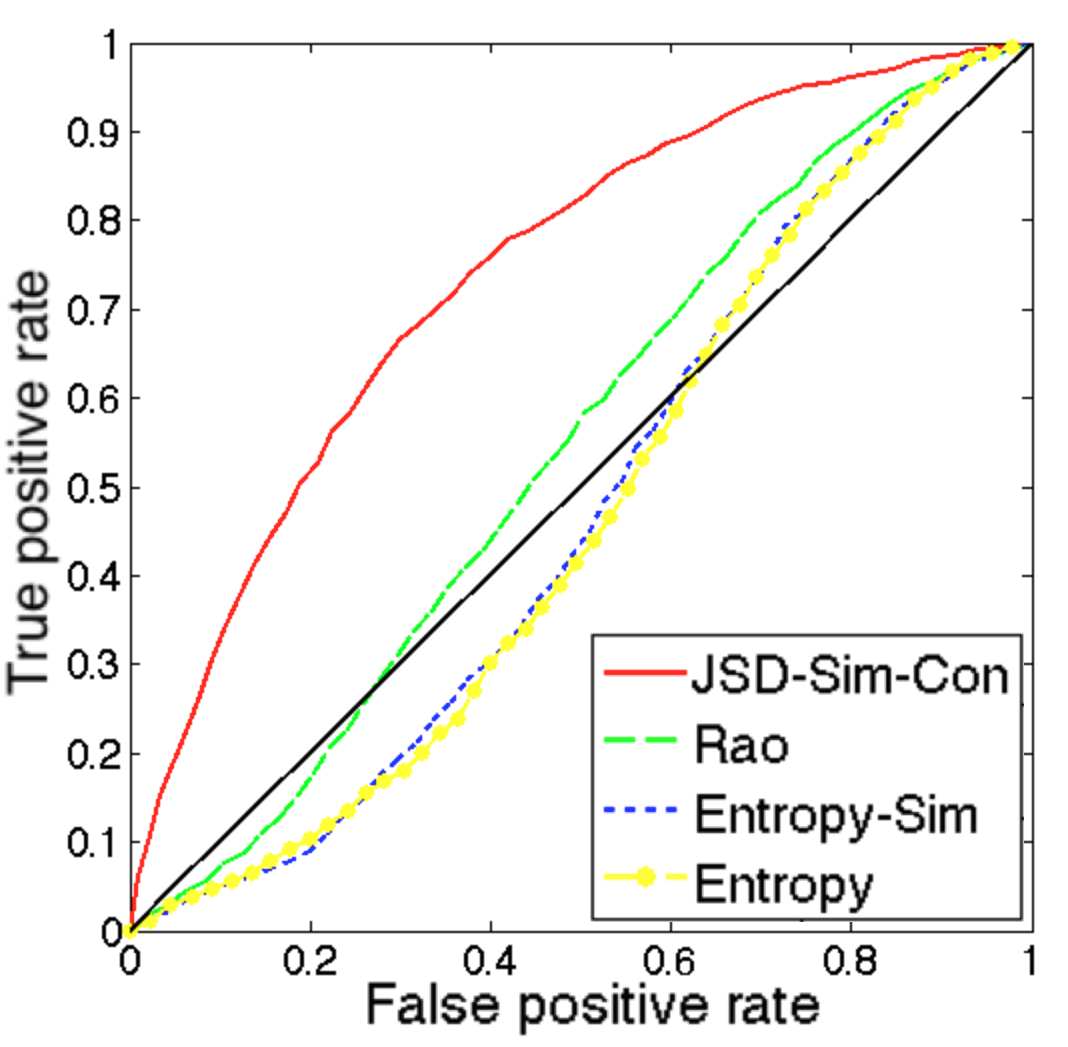
\includegraphics[width=0.24\textwidth]{figures/phonecases-comparison-kopia.png}
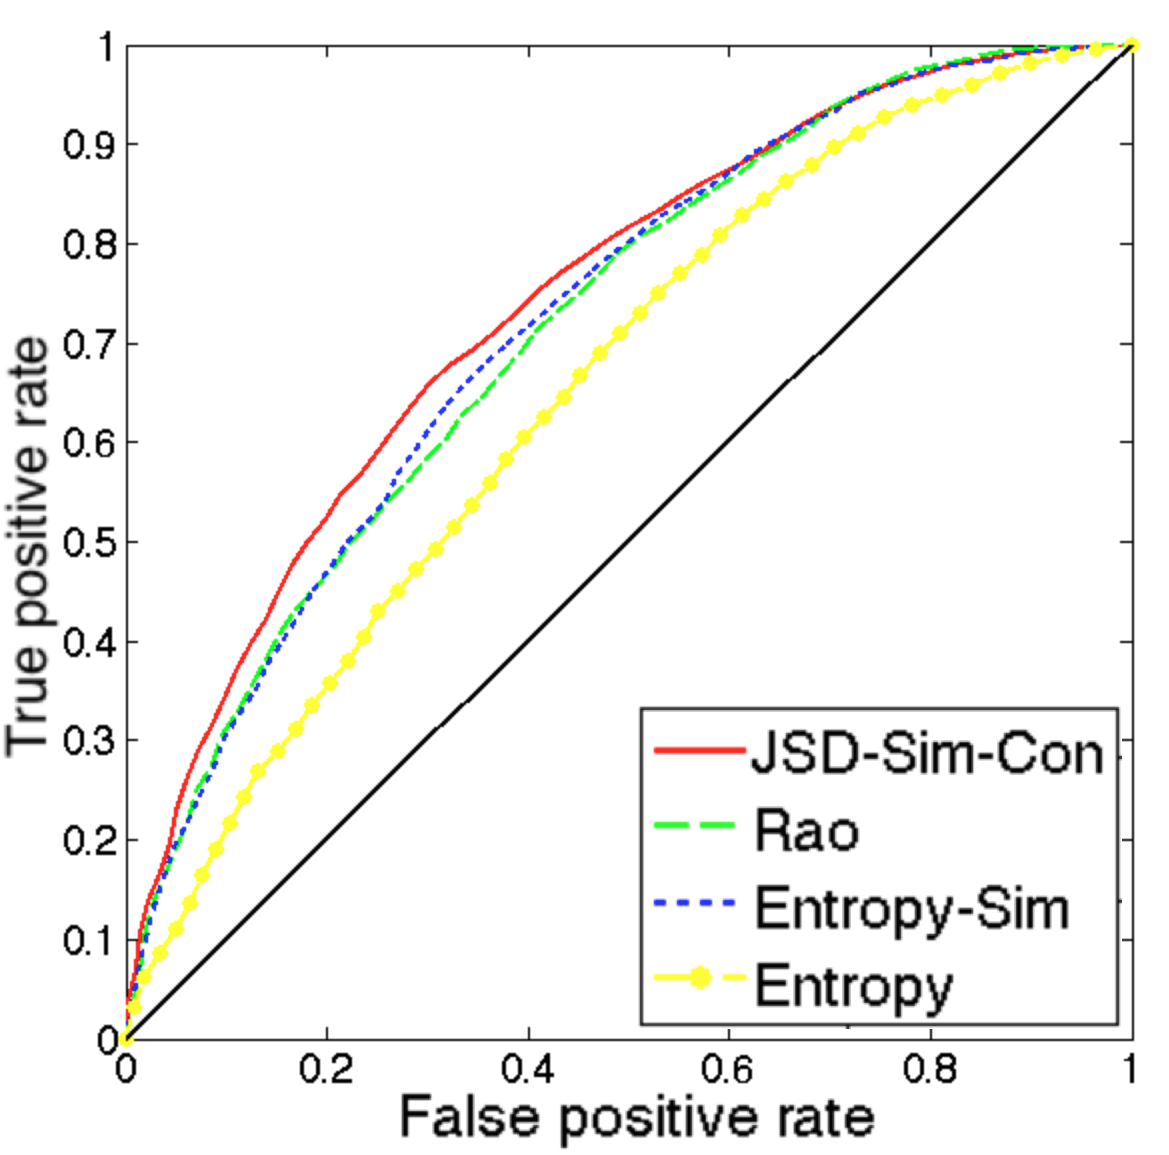
\includegraphics[width=0.24\textwidth]{figures/nsf-comparison-kopia.png}}
{\bf Supervised Results}
\fcolorbox{reddishyellow}{white}{\begin{tabular}{|l|c|c|c|c|}
\hline
&precision & recall & f1 & accuracy
\\ \hline 
JSD         &$\mathbf{0.714}$&$0.597$&$0.650$& $\mathbf{0.8828}$\\
RAE             &$0.676$&$\mathbf{0.666}$&$\mathbf{0.671}$&$0.8809$ \\
LSI             &$0.676$&$0.633$&$0.654$&$0.8778$\\
\hline
\end{tabular}}
\end{center}

\ \\
We draw an ROC curve by thresholding diversity
  over labeled examples. As baselines, we use probabilistic diversity 
  measures with input being an LDA topic distribution for  given
  example:\\
1. Shannon Entropy;\\
2. Shannon Entropy with topic similarities;\\
3. Rao Diversity (also uses topic similarities).

\vspace{3.5em}
We also used the topic vector $\Sigma
D_i \widehat{P}_{W_{\bar{i}}}$ to train an SVM model on eBay data. We
compared this against using feature vectors from:\\ 
1. Recursive Auto-Encoders with Word2Vec;\\
2. Latent Semantic Indexing (LSI).
\end{multicols}
%%%%%%%%%%%%%%%%%%%%%%%%%%%%%%%%%%%%%%%%%%%%%%%%%%%%%%%%%%%%%%%%%%%%%%%%%%%%%%
}


%%%%%%%%%%%%%%%%%%%%%%%%%%%%%%%%%%%%%%%%%%%%%%%%%%%%%%%%%%%%%%%%%%%%%%%%%%%%%%
\headerbox{1. Capturing Topic Similarity}{name=entropy,column=1,below=dms,above=results}{
\fboxsep=2pt
{\bf Problem:} A distributional representation of a word does
  not capture the relations between topics.

\medskip
Using the trained topic model, we can generate a {\bf topic similarity matrix}
  $\cS_{|T|\times|T|}$, where $\cS_{ij}$ indicates
  the degree of similarity between topics $i$ and $j$. We normalize
  the rows of $\cS$ to get distributional vectors.

\vspace{-5mm}\begin{center}\fcolorbox{reddishyellow}{white}{
\parbox{0.95\textwidth}{
Given $P_i$, we can now consider $\tilde{P_i}=P_i\cS^T$, which
  essentially diffuses $P_i$ accross similar topics.
}}\end{center}
%%%%%%%%%%%%%%%%%%%%%%%%%%%%%%%%%%%%%%%%%%%%%%%%%%%%%%%%%%%%%%%%%%%%%%%%%%%%%%
}





\end{poster}

\end{document}
